% +++
% latex="texfot lualatex-dev"
% +++
\documentclass[aspectratio=149,9pt,fleqn]{beamer}
\usetheme[numbering=fraction,block=fill]{metropolis}
\usefonttheme{professionalfonts}

\usepackage{luatexja,luatexja-adjust}
\usepackage[no-math,match,deluxe]{luatexja-fontspec}

\hypersetup{unicode,colorlinks}
\hypersetup{linkcolor=blue,urlcolor=teal,citecolor=olive}
% \hypersetup{linkcolor=black,urlcolor=black,citecolor=black}

\usepackage{pxrubrica}
\usepackage{autobreak}
\usepackage{tikz,pgfplots,tcolorbox}
\usetikzlibrary{calc}
\pgfplotsset{compat=1.16}

\usepackage[version=4,arrows=pgf]{mhchem}
\mhchemoptions{textfontcommand=\sffamily,mathfontcommand=\mathsf}
\newcommand*\cec[1]{\cesplit{{\,\ }{\0}}{#1}}

\usepackage{tabularray}
\SetTblrDefault{rowsep=0pt}

\usepackage[loadonly,]{enumitem}
\newlist{desc}{description}{5}
\setlist[desc]{labelindent=2\zw,labelsep*=1\zw,labelwidth=3\zw}
\newlist{enu}{enumerate}{5}
\setlist[enu]{label*=\arabic*.}

\ltjsetparameter{jacharrange={-2,-3,-8}}
\usepackage[no-math,match,deluxe,fontspec]{luatexja-preset}

% \usepackage[osf]{newpxtext}\usepackage{classico}
\usepackage[nowidering]{yhmath}
\usepackage{newpxmath,amsmath,mathtools,amssymb,mleftright}
\usepackage[T1]{fontenc}
\usepackage[notrig,italicdiff]{physics}
\mleftright

\usepackage[cal=boondoxo,frak=pxtx,bb=ams]{mathalpha}
\DeclareMathAlphabet{\mathnormal}{T1}{pplx}{m}{it}
\DeclareMathAlphabet{\mathrm}{T1}{pplx}{m}{n}
\DeclareMathAlphabet{\mathit}{T1}{pplx}{m}{it}
\DeclareMathAlphabet{\mathtt}{T1}{lmtt}{m}{n}
\DeclareMathAlphabet{\mathsf}{T1}{kurier}{m}{n}
\DeclareMathAlphabet{\mathbsf}{T1}{kurier}{b}{n}
\DeclareMathAlphabet{\mathbold}{T1}{pplx}{b}{it}
\DeclareMathAlphabet{\mathbf}{T1}{pplx}{b}{n}
\DeclareSymbolFont{operators}{T1}{uop}{m}{n}

\DeclareSymbolFont{numbers}{T1}{pplx}{m}{n}
\DeclareMathSymbol{0}\mathalpha{numbers}{`0}
\DeclareMathSymbol{1}\mathalpha{numbers}{`1}
\DeclareMathSymbol{2}\mathalpha{numbers}{`2}
\DeclareMathSymbol{3}\mathalpha{numbers}{`3}
\DeclareMathSymbol{4}\mathalpha{numbers}{`4}
\DeclareMathSymbol{5}\mathalpha{numbers}{`5}
\DeclareMathSymbol{6}\mathalpha{numbers}{`6}
\DeclareMathSymbol{7}\mathalpha{numbers}{`7}
\DeclareMathSymbol{8}\mathalpha{numbers}{`8}
\DeclareMathSymbol{9}\mathalpha{numbers}{`9}

\DeclareFontFamily{U}{mathastro}{}
\DeclareFontShape{U}{mathastro}{m}{n}{<->mathastrotest10}{}
\DeclareSymbolFont{astro}{U}{mathastro}{m}{n}
\DeclareMathSymbol\Sun\mathord{astro}{'300}
\DeclareMathSymbol\Mercury\mathord{astro}{'301}
\DeclareMathSymbol\Venus\mathord{astro}{'302}
\DeclareMathSymbol\Earth\mathord{astro}{'303}
\DeclareMathSymbol\Mars\mathord{astro}{'304}
\DeclareMathSymbol\Jupiter\mathord{astro}{'305}
\DeclareMathSymbol\Saturn\mathord{astro}{'306}
\DeclareMathSymbol\Uranus\mathord{astro}{'307}
\DeclareMathSymbol\Neptune\mathord{astro}{'310}
\DeclareMathSymbol\Pluto\mathord{astro}{'311}
\DeclareMathSymbol\varEarth\mathord{astro}{'312}
\DeclareMathSymbol\Moon\mathord{astro}{'313}
\DeclareMathSymbol\leftmoon\mathord{astro}{'313}
\DeclareMathSymbol\rightmoon\mathord{astro}{'314}
\DeclareMathSymbol\fullmoon\mathord{astro}{'315}
\DeclareMathSymbol\newmoon\mathord{astro}{'316}
\DeclareMathSymbol\newmoon\mathord{astro}{'316}

\setmainfont[
	Ligatures=TeX,
	Scale=0.98,
	BoldFont=FOT-RodinNTLGPro-B,
	ItalicFont=FOT-RodinNTLGPro-B,
]{Palatino}
\setsansfont[
	Ligatures=TeX,
	Scale=0.98,
	BoldFont=FOT-RodinNTLGPro-B,
	BoldItalicFont=FOT-RodinNTLGPro-B,
	%ItalicFont=FOT-RodinNTLGPro-B,
]{Palatino}
\setmainjfont[
	Ligatures=TeX,
	JFM=jlreq,
	BoldFont=FOT-RodinNTLGPro-B,
	ItalicFont=FOT-RodinNTLGPro-B,
]{FOT-ModeMinBLargePro-M}
\setsansjfont[
	Ligatures=TeX,
	JFM=jlreq,
	BoldFont=FOT-RodinNTLGPro-B,
	ItalicFont=FOT-RodinNTLGPro-B,
]{FOT-ModeMinBLargePro-M}
\setmonofont[
	Ligatures=TeXReset,
]{HackGen}
\setmonojfont[
	Ligatures=TeXReset,
]{HackGen}

\allowdisplaybreaks[4]
\ltjenableadjust[lineend=extended,priority=true,profile=true,linestep=false]

%%%%%%%%%%%%自作マクロ
\newcommand{\hmvec}{\mathbold}
\newcommand{\hmeqdef}{\stackrel{\mathrm{def}}{=}}
\newcommand{\hmeqq}{\stackrel{\mathrm{?}}{=}}
\newcommand{\centeralign}[1]{\rule{0pt}{0pt}\hfill#1\hfill\rule{0pt}{0pt}}
\NewDocumentCommand\hmu{s m}{\IfBooleanF{#1}{\,}\ifmmode\mathrm{#2}\else\(\mathrm{#2}\)\fi}
\newcommand{\hmemph}[1]{\textbf{#1}}
\newcommand{\hme}[1]{\times10^{#1}}
\newcommand{\hmfnc}[1]{\(\mathrm{#1}\)}
\newcommand{\hmfconv}{F_\mathrm{conv}}
\NewDocumentCommand\etal{s}{\textit{et al.}\IfBooleanF{#1}{\ }}

\institute{北海道大学大学院理学院 地球流体力学研究室 M2}
\author{人見祥磨}
\title{地球型惑星の射出限界の考察に向けて}
\subtitle{Ishiwatari \etal (2002) のレビュー}

\begin{document}

\maketitle

\begin{frame}
	\frametitle{背景}
	\begin{itemize}
		\item 系外惑星に生命が存在するためには、惑星表面に液体の水があることが
			重要だと考えられる (Kopparapu \etal*, 2013)
		\item 惑星表面に液体の水が存在する条件は、惑星の表面温度が水の
			融点から沸点の間にあることである
		\item 惑星表面に液体の水が存在しうる領域は、ハビタブルゾーン (HZ)と呼ばれる
		\item ここでは HZ の内側の比較的高温な領域で起こる現象に着目する
	\end{itemize}
	\begin{figure}
		\centering\scriptsize
		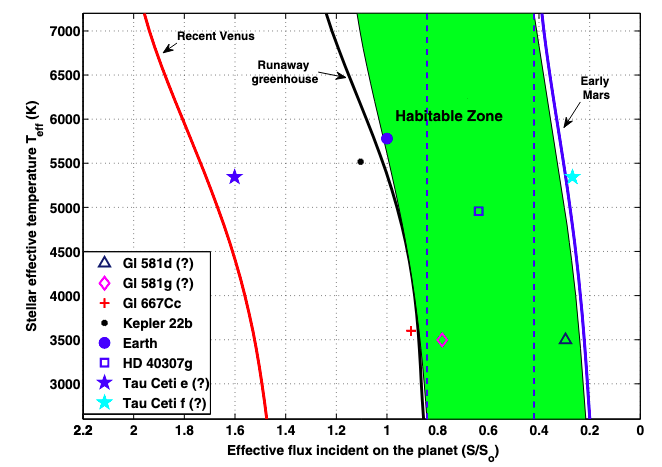
\includegraphics[width=.5\textwidth]{kopparapu8.png}\\
		様々な中心星の有効温度ごとに、雲がない場合の HZ を示したもの。
		(Kopparapu \etal*, 2013; Fig.\ 8)
	\end{figure}
\end{frame}

\begin{frame}
	\frametitle{暴走温室状態}
	\begin{itemize}
		\item HZ の内側境界を決定する重要な概念として、暴走温室状態がある
	\end{itemize}
	\begin{columns}[T,onlytextwidth]
		\begin{column}{.68\textwidth}
			\begin{itemize}
				\item 1990 年以前に次のような暴走温室状態の研究があった
					\begin{itemize}
						\item Plass (1961), Gold (1964)
							\begin{desc}
								\item[思考実験]
								\item[結果] 温度の上昇と水蒸気量の増加には
									正のフィードバックがあり、海洋が完全に蒸発する
							\end{desc}
						\item Komabayashi (1967, 1968), Ingersoll (1969)
							\begin{desc}
								\item[モデル] 灰色成層圏モデル
								\item[結果] 大気上端での外向き赤外放射
									(outgoing longwave radiation: OLR) には上限がある
									(Komabayashi--Ingersoll Limit)
							\end{desc}
						\item Kasting (1988), Abe and Matsui (1988)
							\begin{desc}
								\item[モデル] 鉛直 1 次元放射対流平衡モデル(非灰色)
								\item[結果] OLR には漸近値がある
							\end{desc}
					\end{itemize}
			\end{itemize}
		\end{column}
		\begin{column}{.3\textwidth}
			\centering\scriptsize
			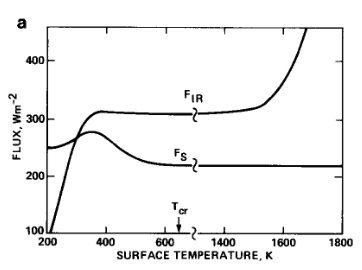
\includegraphics[width=.95\textwidth]{kasting7a.png}\\
			対流圏モデルでの OLR (\(F_{\mathrm{IR}}\)) と\\
			地表面温度の関係\\
			(Kastin, 1988; Fig.\ 7a)
		\end{column}
	\end{columns}
	\begin{itemize}
		\item Komabayashi--Ingersoll Limit と Kasting, Abe and Matusi の
			漸近値の対応が明確ではなかった
		\item 暴走温室状態や OLR の上限について、Nakajima \etal (1992) が整理を行った
	\end{itemize}
\end{frame}

\begin{frame}
	\frametitle{Nakajima \etal (1992) のレビュー}
	\begin{desc}
	\item[モデル] 鉛直 1 次元放射対流平衡モデル
			\begin{table}
				\tiny
				\begin{tblr}{rl}
					\hline
					&Nakajima \etal (1992) モデル設定\\
					\hline
					成層圏&放射平衡\\
					対流圏界面&飽和水蒸気\\
					対流圏&湿潤擬断熱減率\\
					大気成分&2 成分(水蒸気、乾燥空気)、理想気体、分子量同じ\\
					放射過程&散乱なし、灰色\\
					水蒸気の吸収係数&\(\kappa_v=0.01\hmu{m^2/kg}\)\\
					乾燥空気の吸収係数&\(\kappa_n=0\)\\
					\hline
				\end{tblr}
			\end{table}
	\end{desc}
	\begin{columns}[T,onlytextwidth]
		\begin{column}{.6\textwidth}
			\begin{desc}
				\item[結果]\leavevmode
					\begin{itemize}
						\item OLR には、水蒸気の乾燥空気に対する割合に応じて、
							3 種類の上限がある
						\item 水蒸気の割合が少ないときの上限\\
							(Komabayashi--Ingersoll Limit)
						\item 水蒸気の割合が多くないときの上限\\
							(対流圏の構造による上限)
						\item 水蒸気のみの大気の上限\\
							(Kastingや Abe and Matsui の漸近値に対応)
					\end{itemize}
			\end{desc}
		\end{column}
		\begin{column}{.38\textwidth}
			\begin{figure}
				\scriptsize
				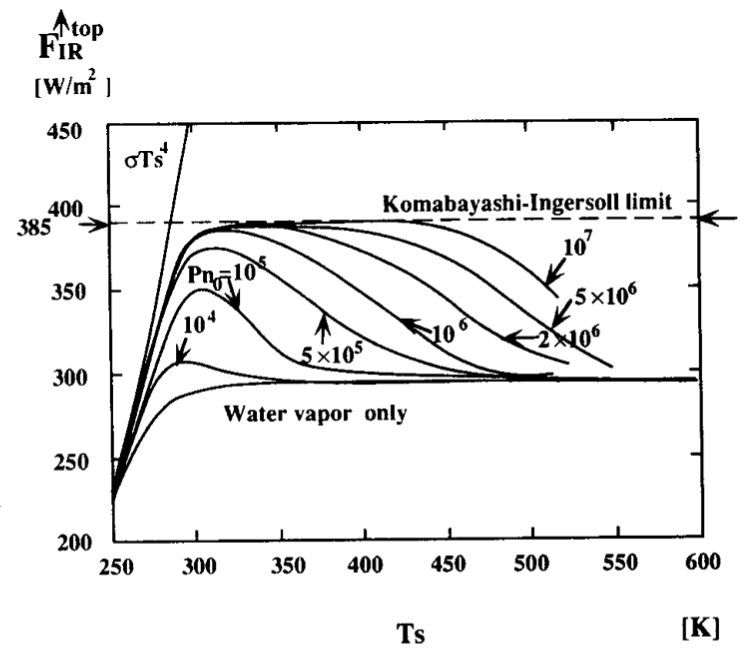
\includegraphics[width=\textwidth]{nf6.png}\\
				地表面での乾燥空気の分圧 \(p_{n0}\) を変えた時の\\
				地表面温度と OLR の関係\\
				(Nakajima \etal*, 1992; Fig.\ 6)
			\end{figure}
		\end{column}
	\end{columns}
\end{frame}

\begin{frame}
	\frametitle{Ishiwatari \etal (2002) の目的}
	\begin{desc}
		\item[目的]\leavevmode
			\begin{itemize}
				\item 3 次元系でも射出限界が現れるか確認するのが目的
					\begin{itemize}
						\item 1 次元モデルの射出限界は 3 次元ではあらわれない可能性がある
							\begin{itemize}
								\item 3 次元系では、循環の効果を考える必要がある
								\item 太陽定数が大きくなると循環は強まる
								\item 循環が強くなると、ハドレー循環下降域である
									亜熱帯で乾燥化が進む可能性がある
								\item 亜熱帯で乾燥化が進むと、大気が光学的に薄くなり、
									そこから暴走しないように射出される可能性がある
							\end{itemize}
					\end{itemize}
				\item 射出限界があらわれるならば暴走温室状態になるが、
					暴走温室状態ではどのようなことが起こるか
			\end{itemize}
		\item[行ったこと]\leavevmode
			\begin{itemize}
				\item Nakajima \etal (1992) の枠組みを踏まえ GCM 計算を行う
					\begin{itemize}
						\item 地球的な大規模循環ができるような計算を行う
							\begin{itemize}
								\item 地球を模した入射するエネルギーフラックス
									(surface shortwave radiation: SSR)
									の緯度分布を与える
							\end{itemize}
						\item 平衡解が存在しない場合の振る舞いを検討できる
							\begin{itemize}
								\item 時間発展計算を行う
							\end{itemize}
					\end{itemize}
			\end{itemize}
	\end{desc}
\end{frame}

\begin{frame}
	\frametitle{モデル}
	\begin{itemize}
		\item 利用したモデル
			\begin{itemize}
				\item AGCM5
			\end{itemize}
		\item 基礎方程式
			\begin{itemize}
				\item 以下の 3 次元球殻上プリミティヴ方程式
			\end{itemize}
	\end{itemize}
	\tiny
	\begin{gather*}
		\dv{\zeta}{t}=-\frac{1}{a\cos\varphi}\pdv{}{\lambda}
		\qty[-(\zeta+f)u-\dot\sigma\pdv{u}{\sigma}-\frac{RT'}{a\cos\varphi}\pdv{\pi}{\lambda}]
		-\frac{1}{a\cos\varphi}\pdv{}{\varphi}
		\qty[\qty((\zeta+f)v-\dot\sigma\pdv{u}{\sigma}-
		\frac{RT'}{a}\pdv{\pi}{\varphi})\cos\varphi]
		-F_\zeta^\mathit{diff},\tag{渦度}\\
		\dv{D}{t}=\frac{1}{a\cos\varphi}\pdv{}{\lambda}
		\qty[(\zeta+f)v-\dot\sigma\pdv{u}{\sigma}-x\frac{RT'}{a}\pdv{\pi}{\varphi}]
		+\frac{1}{a\cos\varphi}\pdv{}{\varphi}
		\qty[\qty((\zeta+f)v-\dot\sigma\pdv{u}{\sigma}-
		\frac{RT'}{a}\pdv{\pi}{\varphi})\cos\varphi]
		-\nabla^2(\Phi+R\bar T\pi+E)-F_D^\mathit{diff},\tag{発散}\\
		\dv{\pi}{t}=-\frac{1}{a\cos\varphi}\pdv{u}{\lambda}
		-\frac{1}{a\cos\varphi}\pdv{}{\varphi}[v\cos\varphi]-\pdv{\dot\sigma}{\sigma},\quad
		\pdv{\Phi}{\sigma}=-\frac{RT}{\sigma},\quad
		\dv{q}{t}=\frac{g}{p_s}\pdv{F_q^\mathit{vdf}}{\sigma}+F_q^\mathit{vdf}+S_q^\mathit{cond},
		\tag{連続の式, 静水圧, 比湿}\\
		\dv{T}{t}=\frac{RT}{c_p}\qty(\pdv{\pi}{t}+\frac{u}{a\cos\varphi}\pdv{\pi}{\lambda}+
		\frac{v}{a}\pdv{\pi}{\varphi}+\frac{\dot\sigma}{\sigma})
		+\frac{1}{c_p}\qty(\frac{g}{p_s}\pdv{F_T^\mathit{vdf}}{\sigma}+
		\frac{g}{p_s}\pdv{F_\mathrm{rad}^\mathit{vdf}}{\sigma})
		+F_T^\mathit{diff}+LS_q^\mathit{cond},\tag{熱力学}\\
		\dv{}{t}
		\equiv\pdv{}{t}+\frac{u}{a\cos\varphi}\pdv{}{\lambda}
		+\frac{u}{a}\pdv{}{\varphi}+\dot\sigma\pdv{}{\sigma},\quad
		\zeta\equiv\frac{1}{a\cos\varphi}\pdv{v}{\lambda}
		-\frac{1}{a\cos\varphi}\pdv{}{\varphi}[u\cos\varphi],\\
		D\equiv\frac{1}{a\cos\varphi}\pdv{u}{\lambda}
		+\frac{1}{a\cos\varphi}[v\cos\varphi],\quad
		\Phi\equiv gz,\quad\pi\equiv\ln p_s
	\end{gather*}
	\((\lambda,\varphi)\): 緯度経度; \(\sigma\): 高度(\(\sigma\) 座標); \(u, v\): 水平風;
	\(\dot\sigma\): \(\sigma\) 座標での鉛直風; \(T\): 温度; \(q\): 比湿;
	\(p_s\): 地表面気圧; \(f\): コリオリパラメータ; \(a\): 惑星半径; \(g\): 重力加速度;\\
	\(R\): 乾燥空気の気体定数; \(c_p\): 定圧比熱; \(L\): 水の潜熱;
	\(F_\bullet^\mathit{diff}\): 水平拡散項; \(F_\bullet^\mathit{vdf}\): 鉛直拡散項;
	\(S_q^\mathit{cond}\): 結露・凝結による比湿の変化;
\end{frame}

\begin{frame}
	\frametitle{大気成分と物理過程}
	\begin{itemize}
		\item 大気成分
			\begin{itemize}
				\item 大気は凝結性成分(水蒸気)と非凝結性成分(乾燥空気)からなる
				\item 両成分とも分子量が同じであるとする
			\end{itemize}
		\item 物理過程
	\end{itemize}
	\begin{columns}[onlytextwidth,T]
		\begin{column}{.05\textwidth}
		\end{column}
		\begin{column}{.45\textwidth}
			\begin{itemize}
				\item 積雲過程
					\begin{itemize}
						\item 湿潤対流調節スキーム (Manabe \etal*, 1965)
							\begin{itemize}
								\item 上下 2 層で湿潤不安定が起きている場合に適用
								\item 気温減率を湿潤断熱減率に変更する
							\end{itemize}
					\end{itemize}
				\item 大規模凝結過程
				\item 放射過程 (Nakajima \etal*, 1992)
					\begin{itemize}
						\item 水蒸気のみが長波放射を吸収し、
							吸収係数は一定である
					\end{itemize}
				\item 鉛直混合 (Yamada and Mellor, 1974)
			\end{itemize}
		\end{column}
		\begin{column}{.45\textwidth}
			\begin{itemize}
				\item 地表面フラックス (Louis, 1979)
				\item 強い人工散逸
					\begin{itemize}
						\item レイリー散逸、ニュートン冷却、鉛直フィルターを導入した
						\item 導入した理由は、計算不安定を発生させないため
						\item 試計算では内部重力波が増幅し、計算不安定が起きた
						\item ハドレー循環や傾圧不安定などの対流圏の大気循環の基本的な
							構造は表現されているので、大きな影響はないとした
					\end{itemize}
			\end{itemize}
		\end{column}
	\end{columns}
\end{frame}

\begin{frame}
	\frametitle{実験設定}
	\begin{columns}[T,onlytextwidth]
		\begin{column}{.5\textwidth}
			\begin{itemize}
				\item 地表面で熱バランスが成り立ち、湿り度は 1 とする(すべて海で覆われている)
				\item 分解能
					\begin{itemize}
						\item 水平方向はスペクトル法で計算
							\begin{itemize}
								\item 水平分解能は三角形切断の T21 に対応した \(32\times64\)
							\end{itemize}
						\item 鉛直方向は差分法で計算
							\begin{itemize}
								\item 層数は 32
							\end{itemize}
					\end{itemize}
				\item 太陽定数 \(S\) を変化させて実験を行った
					\begin{itemize}
						\item 実験した太陽定数は表の 8 つ。実験名の S の後ろが太陽定数
						\item 実験 S1380 が現在の地球に相当
					\end{itemize}
					\begin{table}
						\scriptsize
						\begin{tblr}{c|cccc}
							\hline
							実験名&S1200&S1380&S1500&S1550\\
							\hline
							SSR(\hmu*{W/m^2})&300.0&345.0&375.0&387.5\\
							\hline
							\hline
							実験名&S1570&S1600&S1700&S1800\\
							\hline
							SSR(\hmu*{W/m^2})&392.5&400.0&425.0&450.0\\
							\hline
						\end{tblr}
					\end{table}
				\item 初期条件
					\begin{itemize}
						\item 静止、等温 (\(280\hmu{K}\))、比湿一様 (\(10^{-3}\))
					\end{itemize}
			\end{itemize}
		\end{column}
		\begin{column}{.45\textwidth}
			\begin{table}
				\tiny
				\begin{tblr}{rl}
					\hline
					&モデルの変数\\
					\hline
					気体定数&\(R=8.314\hmu{J/kg/K}\)\\
					重力加速度&\(g=9.8\hmu{m/s^2}\)\\
					\hline
					非凝縮成分の分子量&\(m_n=18\hme{-3}\hmu{kg/mol}\)\\
					凝縮成分の分子量&\(m_v=18\hme{-3}\hmu{kg/mol}\)\\
					凝縮成分の定圧モル比熱&\(c_{pv}=3.5R\)\\
					非凝縮成分の定圧モル比熱&\(c_{pn}=3.5R\)\\
					凝縮成分の潜熱&\(L=2.4253\hme{6}\hmu{J/kg}\)\\
					地表面での非凝縮成分の量&\(p_{n0}=10^5\hmu{Pa}\)\\
					凝縮成分の吸収係数&\(\kappa_v=0.01\hmu{m^2/kg}\)\\
					非凝縮成分の吸収係数&\(\kappa_n=0\hmu{m^2/kg}\)\\
					\hline
					地表面の比熱&\(0\)\\
					地表面のアルベド&\(0\)\\
					\hline
				\end{tblr}
			\end{table}
			\begin{center}
				\scriptsize
				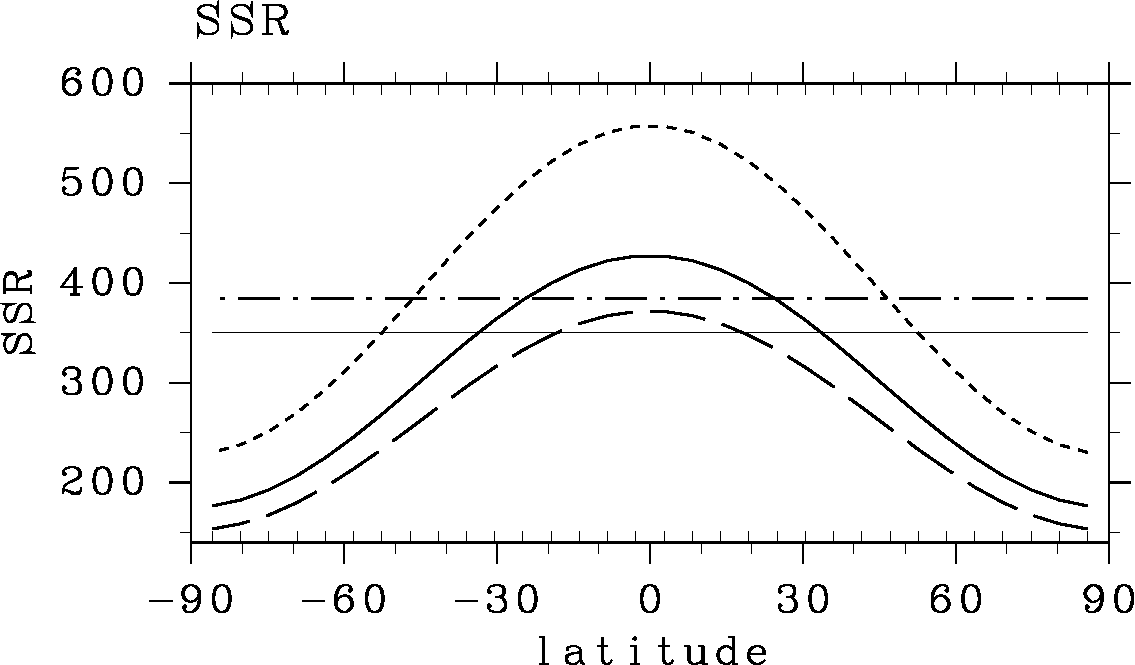
\includegraphics[width=.7\textwidth]{./fig/SSR.kps-crop.pdf}\\
				モデルに与える SSR 緯度分布と\\
				Komabayashi--Ingersoll limit,\\
				及び Nakajima \etal (1992) で得られた放射上限 (\hmu*{W/m^2})\\
				(Ishiwatari \etal*, 2002; Fig.~1)
			\end{center}
		\end{column}
	\end{columns}
\end{frame}

\begin{frame}
	\frametitle{熱的暴走状態の発生}
	{\footnotesize
		Ishiwatari \etal (2002) にバグがあったため、
		後に示す大気の循環構造については注意して見ていただきたい。
	}
%	\begin{itemize}
%		\item いくつかの実験で、全球平均の地表面温度と OLR の時間変化を見る
%			\begin{figure}
%				\scriptsize
%				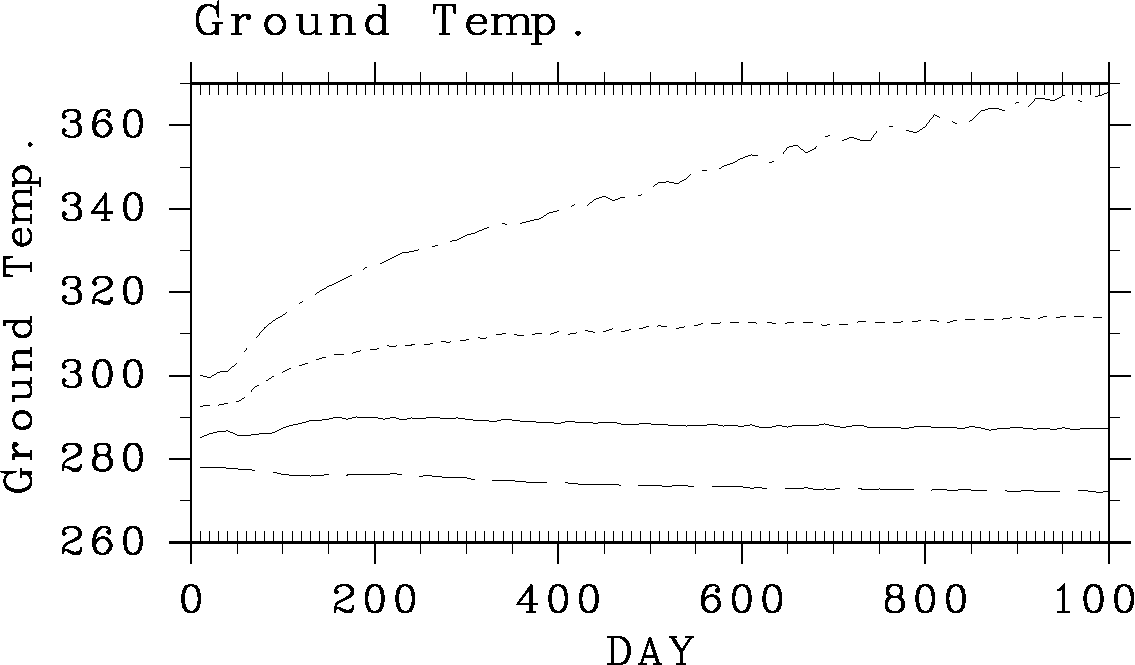
\includegraphics[width=.35\textwidth]{./fig/Tg-seqs.kps-crop.pdf}
%				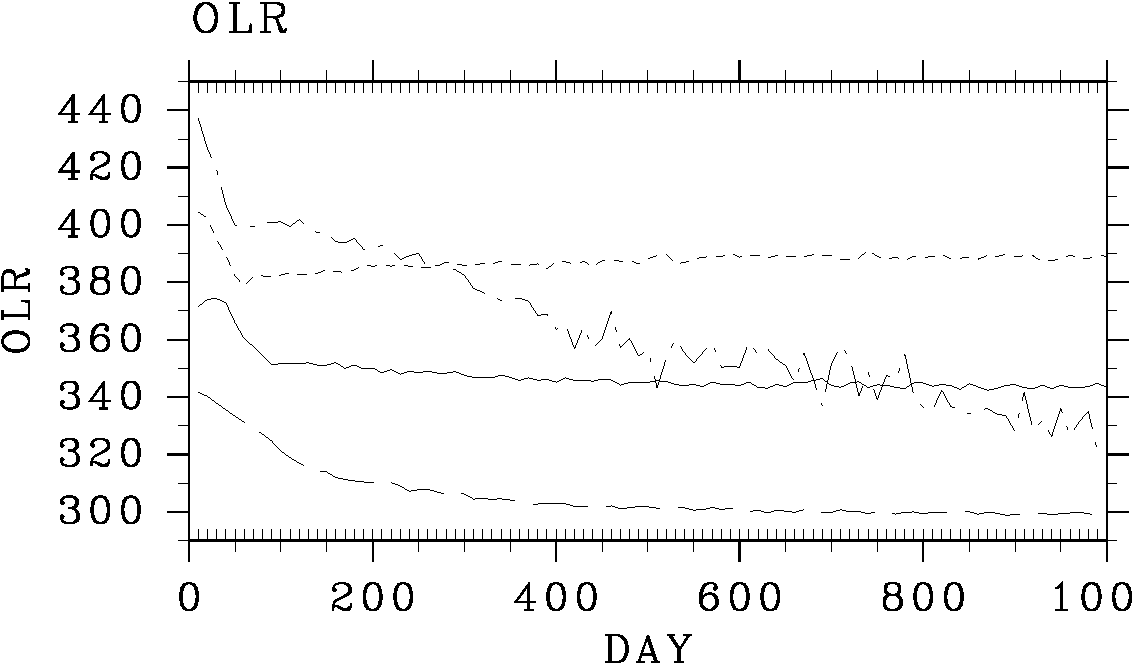
\includegraphics[width=.35\textwidth]{./fig/OLR-seqs.kps-crop.pdf}\\
%				全球平均 OLR (\hmu*{W/m^2}) と全球平均表面温度 (\hmu*{K}) の時間変化;
%				S1200, S1380, S1570, S1800 の結果 (Ishiwatari \etal*, 2002; Fig.~2)
%			\end{figure}
%			\begin{itemize}
%				\item \(S\leq1570\hmu{W/m^2}\) の場合、平衡状態になる
%				\item \(S=1800\hmu{W/m^2}\) の場合、熱的暴走する
%					\begin{itemize}
%						\item OLR は減少し続け、表面温度は増加し続ける
%					\end{itemize}
%			\end{itemize}
%	\end{itemize}
	\begin{columns}[T,onlytextwidth]
		\begin{column}{.6\textwidth}
			\begin{itemize}
				\item いくつかの実験での全球平均の地表面温度と OLR の時間変化
					(右 2 図)
					\begin{itemize}
						\item \(S\leq1570\hmu{W/m^2}\) の場合、平衡状態になる
						\item \(S=1800\hmu{W/m^2}\) の場合、熱的暴走する
							\begin{itemize}
								\item OLR は減少し続け、表面温度は増加し続ける
							\end{itemize}
					\end{itemize}
				\item 全ての実験結果での SSR, OLR の関係(下図)
					\begin{itemize}
						\item \(S>1600\hmu{W/m^2}\) では平衡状態にならない
					\end{itemize}
					\begin{figure}
						\scriptsize
						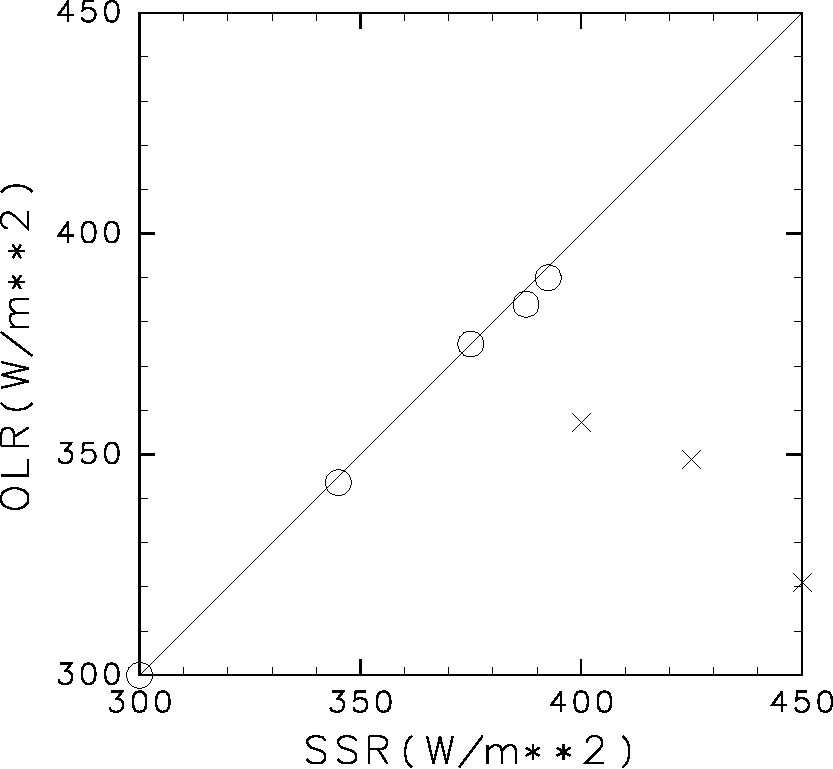
\includegraphics[width=.4\textwidth]{./fig/ISR-OLR.kps-crop.pdf}\\
						全ての実験での SSR, OLR の関係; ◯では熱的平衡、×印では熱的暴走\\
						積分時間は 1000 日(S1600 のみ 2000 日) (Ishiwatari \etal*, 2002; Fig.~3)
					\end{figure}
			\end{itemize}
		\end{column}
		\begin{column}{.4\textwidth}
			\scriptsize
			\begin{figure}
				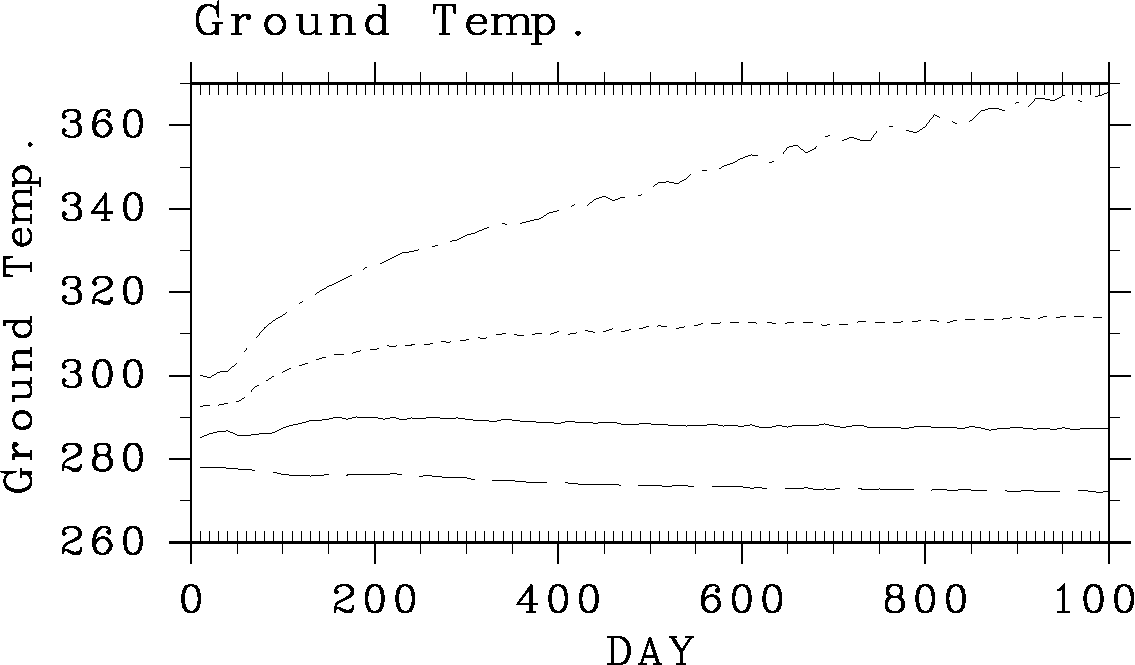
\includegraphics[width=.9\textwidth]{./fig/Tg-seqs.kps-crop.pdf}\\
				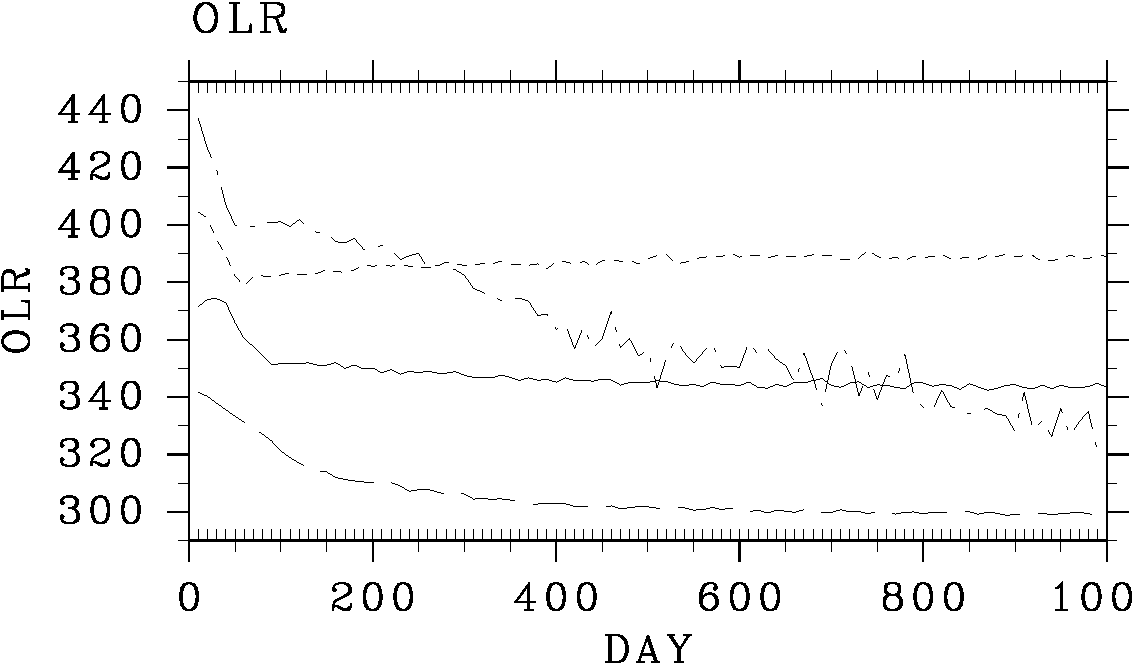
\includegraphics[width=.9\textwidth]{./fig/OLR-seqs.kps-crop.pdf}\\
				全球平均 OLR (\hmu*{W/m^2}) と全球平均表面温度 (\hmu*{K}) の\\
				時間変化; S1200, S1380, S1570, S1800 の結果\\
				(Ishiwatari \etal*, 2002; Fig.~2)
			\end{figure}
		\end{column}
	\end{columns}
\end{frame}

\begin{frame}
	\frametitle{OLR と表面温度の南北分布}
	\begin{columns}[T,onlytextwidth]
		\begin{column}{.55\textwidth}
			\begin{itemize}
				\item 赤道付近の OLR は約 \(390\hmu{W/m^2}\) で頭打ち
				\item 中高緯度の OLR は太陽定数の増加に伴って \(400\hmu{W/m^2}\) に漸近
					\begin{itemize}
						\item 上限のようなものが現れる
						\item 3 次元モデルでの上限値は \(400\hmu{W/m^2}\) に見える
					\end{itemize}
				\item 東西平均地表面温度も OLR と同様に平坦化の傾向
					\begin{itemize}
						\item 地表面温度の南北差が減る
						\item 1 次元的に扱えるかもしれない
					\end{itemize}
				\item GCM で得られたこの上限値が 1 次元モデルの上限と対応するか考察する
			\end{itemize}
		\end{column}
		\begin{column}{.4\textwidth}
			\centering
			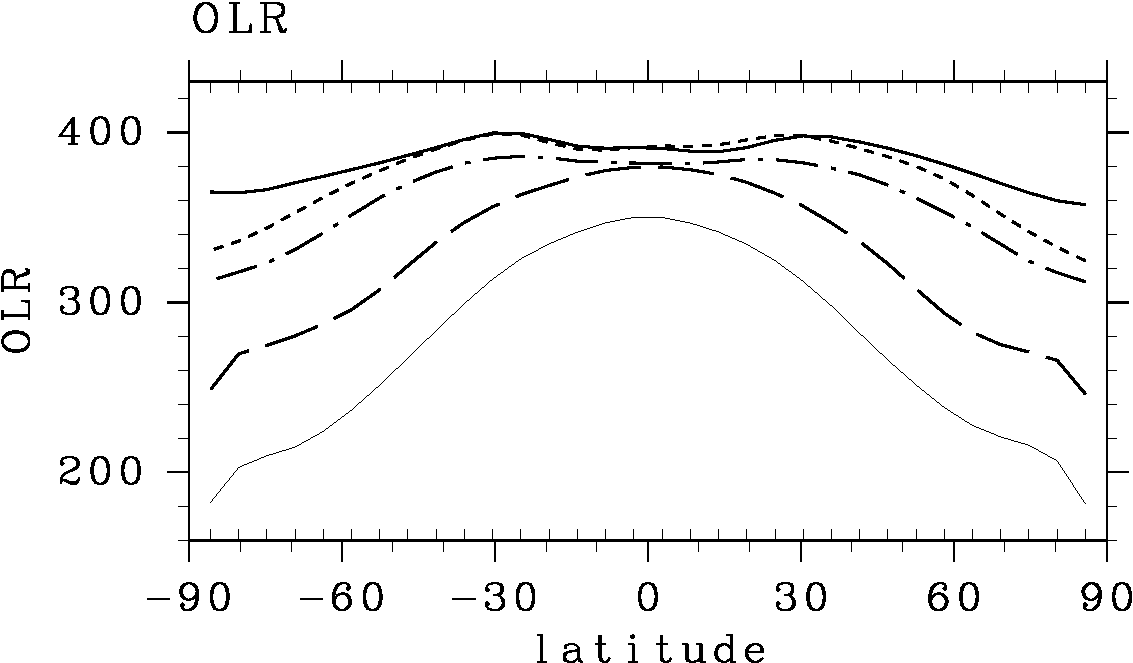
\includegraphics[width=\textwidth]{./fig/OLR-meris.kps-crop.pdf}\\
			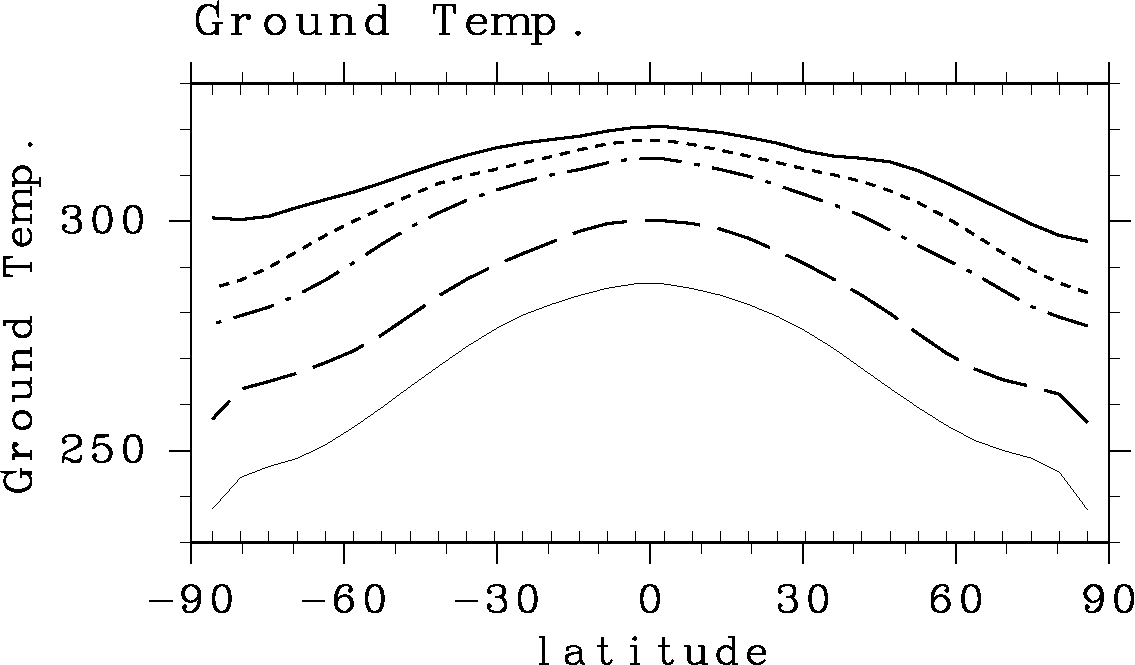
\includegraphics[width=\textwidth]{./fig/Tg-meris.kps-crop.pdf}\\
			\scriptsize Ishiwatari \etal (2002) Fig.\ 4\\
			平衡状態における OLR と東西平均値表面温度\\
			実験 S1570, S1550, S1500, S1380, S1200 の結果
		\end{column}
	\end{columns}
\end{frame}

\begin{frame}
	\frametitle{1 次元系との比較---Komabayashi--Ingersoll Limit}
	\begin{itemize}
		\item Komabayashi--Ingersoll Limit (\(385\hmu{W/m^2}\)) は圏界面が飽和しているときの上限
			\begin{itemize}
				\item 3 次元系と比較するためには、圏界面の相対湿度
					\(\mathit{Rh}\) を調べる必要がある
			\end{itemize}
		\item 実験 S1570 では、圏界面の \(\mathit{Rh}\) は \(50\hmu{\%}\) 程度
			\textcolor[cmyk]{1,1,0,0}{(青線)}
			\begin{center}
				\scriptsize
				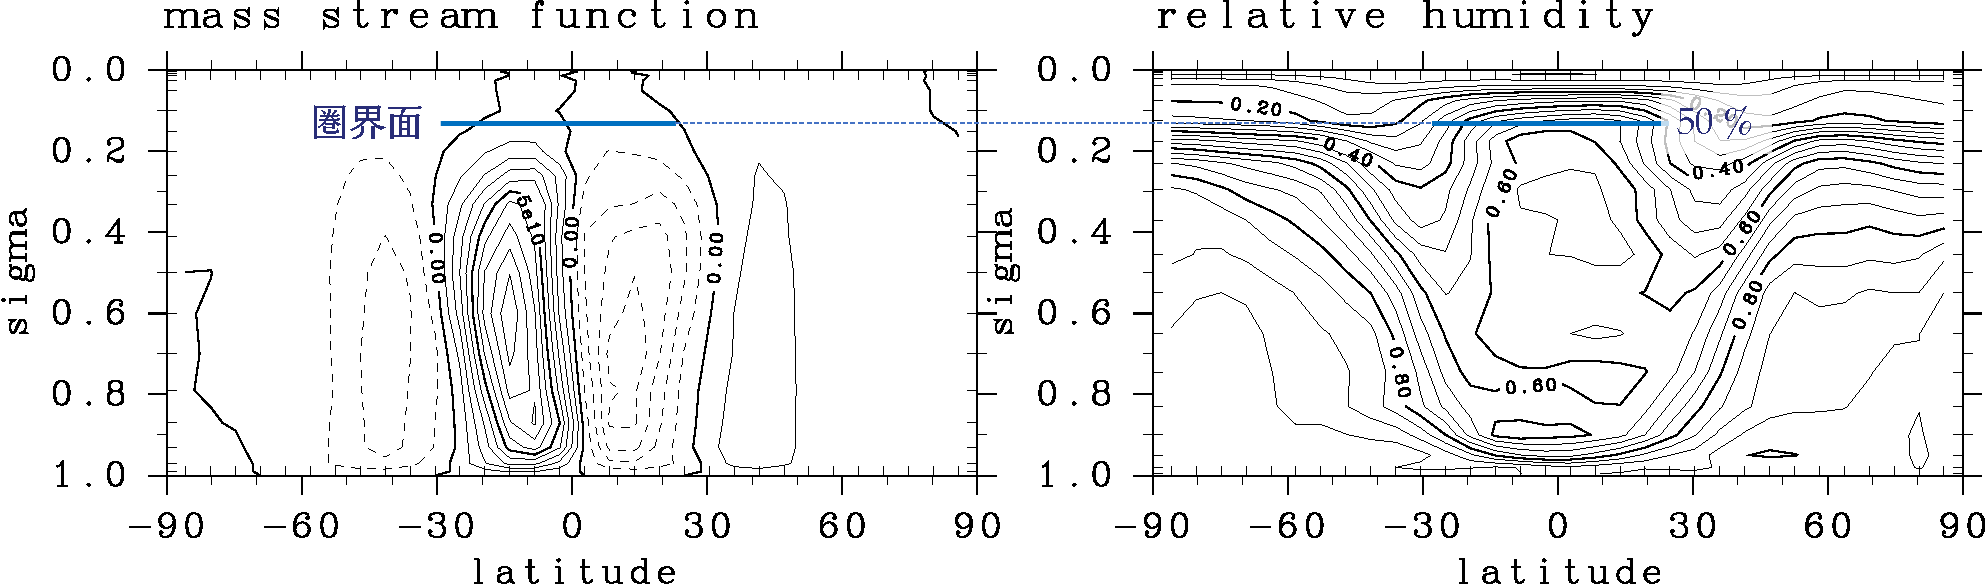
\includegraphics[width=.7\textwidth]{zu-ao.pdf}\\
				実験 S1570 の子午面構造;
				質量流線関数と \(\mathit{Rh}\)  (Ishiwatari \etal*, 2002; Fig.\ 9)
			\end{center}
		\item \(\mathit{Rh}=50\hmu{\%}\) の
			Komabayashi--Ingersoll limit を計算すると約 \(450\hmu{W/m^2}\) になり、
			GCM で得た上限より大きい
			\begin{itemize}
				\item \(\mathit{Rh}\) に応じて圏界面の光学的深さを浅くして求める
			\end{itemize}
		\item GCM で得られた上限と Komabayashi--Ingersoll Limit とは対応していないと考えられる
	\end{itemize}
\end{frame}

\begin{frame}
	\frametitle{1 次元系との比較---対流圏の構造による上限}
	\begin{itemize}
		\item Nakajima \etal (1992) が得た上限 (\(350\hmu{W/m^2}\)) は対流圏が飽和しているときの上限
			\begin{itemize}
				\item 3 次元系と比較するためには、圏界面の \(\mathit{Rh}\) を調べる必要がある
			\end{itemize}
		\item 実験 S1570 では、赤道域対流圏 \(\mathit{Rh}\) は \(60\hmu{\%}\) 程度
			\textcolor[cmyk]{0,1,1,0}{(赤線)}
			\begin{center}
				\scriptsize
				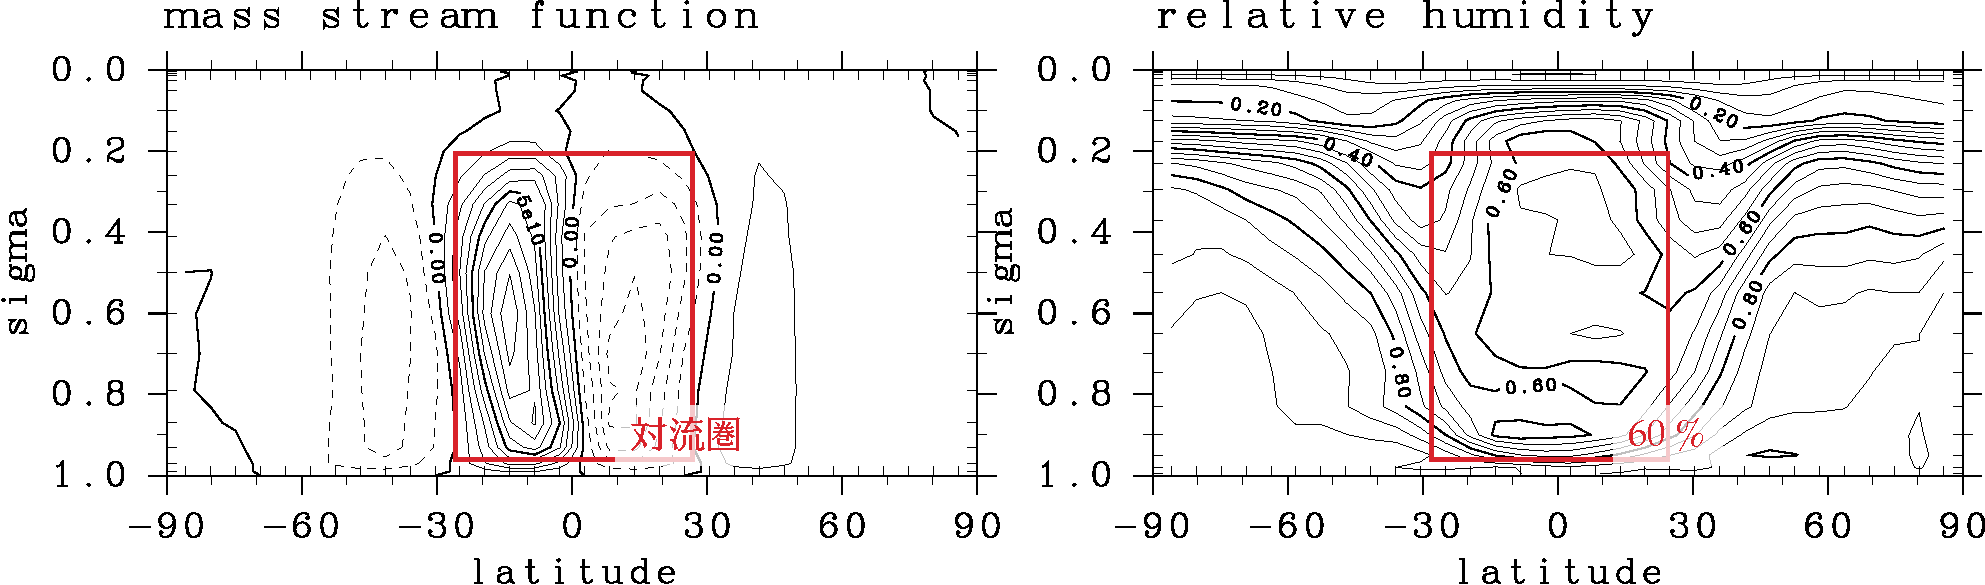
\includegraphics[width=.7\textwidth]{zu-aka.pdf}\\
				実験 S1570 の子午面構造;
				質量流線関数と \(\mathit{Rh}\)  (Ishiwatari \etal*, 2002; Fig.\ 9)
			\end{center}
	\end{itemize}
	\begin{columns}[T,onlytextwidth]
		\begin{column}{.48\textwidth}
			\begin{itemize}
				\item 大気の \(\mathit{Rh}\) を \(60\hmu{\%}\) に固定して、1 次元放射対流平衡モデルで
					放射上限を計算すると、\(385\hmu{W/m^2}\) になり、GCM で得た上限に近い
				\item GCM で得られた上限値と
					Nakajima \etal (1992) が得た上限はに対応しているといえる
			\end{itemize}
		\end{column}
		\begin{column}{.5\textwidth}
			\begin{figure}
				\scriptsize
				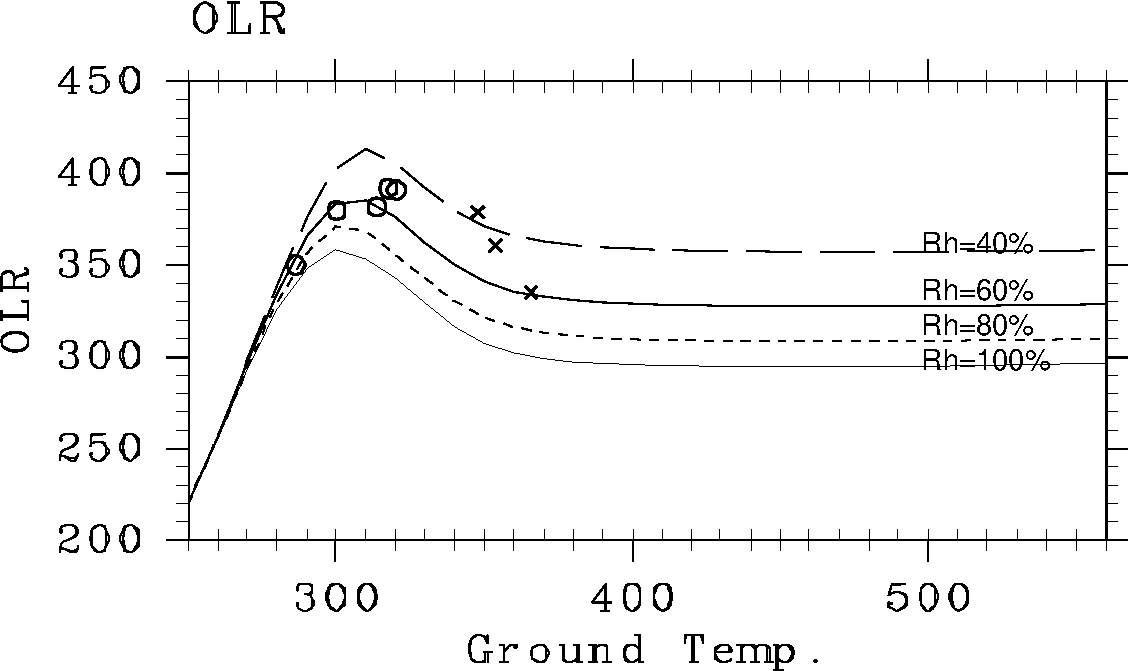
\includegraphics[width=.7\textwidth]{./fig/Tg-OLR-1dimL99-3dEq-crop.pdf}\\
				\hmemph{曲線}: \(\mathit{Rh}\) を変化させた時の1 次元放射対流平衡計算の結果\\
				\hmemph{○×印}: 3 次元計算での赤道東西平均の OLR と 地表面温度の関係\\
				(Ishiwatari \etal*, 2002; Fig.~7)
			\end{figure}
		\end{column}
	\end{columns}
\end{frame}

%\begin{frame}
%	\frametitle{循環構造}
%	\begin{columns}
%		\begin{column}{.4\textwidth}
%		\end{column}
%		\begin{column}{.6\textwidth}
%		\end{column}
%	\end{columns}
%\end{frame}

\begin{frame}
	\frametitle{Ishiwatari \etal (2002) の結論}
	\begin{itemize}
		\item Nakajima \etal (1992) の枠組みを拡張して 3 次元系で数値計算を行った
		\begin{itemize}
			\item 3 次元計算でも放射上限が現れる
				\begin{itemize}
					\item 暴走温室状態になる程度にしか亜熱帯は乾燥しない
					\item 大気が射出できる OLR の上限はおよそ \(400\hmu{W/m^2}\)
						(太陽定数にして \(1600\hmu{W/m^2}\))
					\item この上限は Nakajima \etal (1992) で示された対流圏の構造によって与えられる
						放射上限に対応する
				\end{itemize}
			\item この上限を超えたフラックスが入射すると、大気は熱的に暴走する
				\begin{itemize}
					\item 熱的に暴走すると、OLR は減り、 SSR と OLR の差が拡大する
				\end{itemize}
		\end{itemize}
	\end{itemize}
\end{frame}

\begin{frame}
	\frametitle{Ishiwatari \etal (2002) に含まれるバグ}
	\begin{itemize}
		\item Ishiwatari \etal (2002) にはバグが含まれていた (Ishiwatari \etal*, 2021)
			\begin{itemize}
				\item 湿潤対流調節スキームが動作する条件が逆になっていた
					\begin{itemize}
						\item 鉛直成層が湿潤断熱減率よりも安定しているときに対流調節が働くようになっていた
					\end{itemize}
				\item 長期間(数万日)の積分が実行できない
				\item バグによって計算結果が変わっていそう
			\end{itemize}
	\end{itemize}
	\begin{figure}
		\centeralign{\fbox{オリジナル}\hfill\fbox{バグ修正後}}\\
		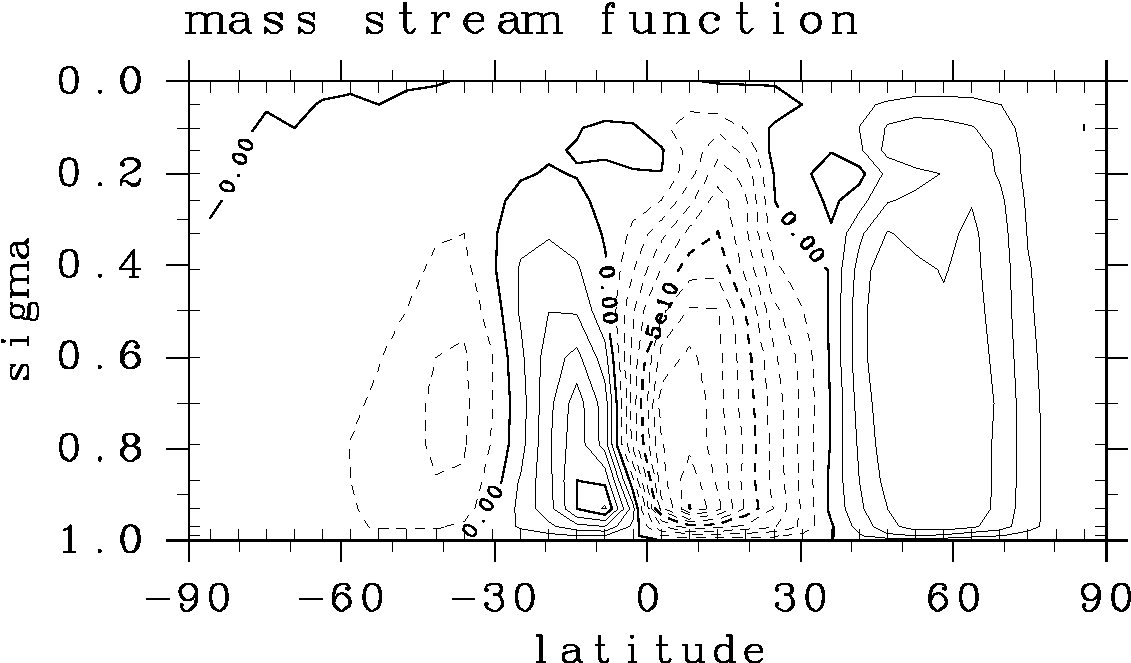
\includegraphics[height=8\zh]{S1380-Strm-crop.pdf}
		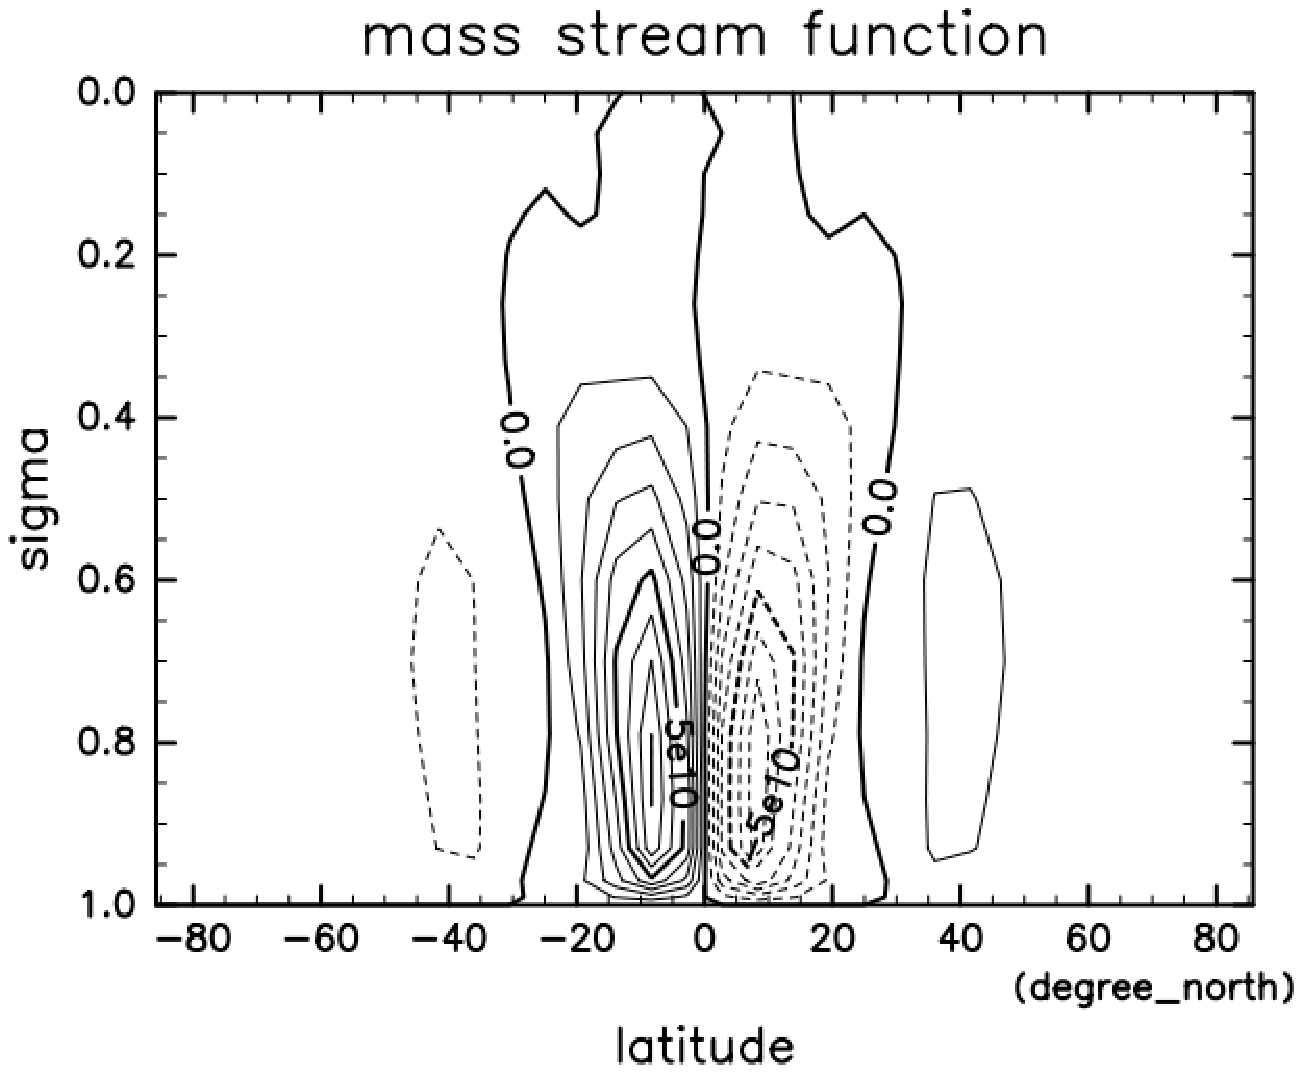
\includegraphics[height=8\zh]{Fig4b_MSF_S1380.pdf}\\
		\scriptsize
		Ishiwatari \etal (2021) で行われた、バグを修正すると計算結果がどれだけ
		変わるかを示す図(質量流線関数の図)
	\end{figure}
\end{frame}

\begin{frame}
	\frametitle{今後の展望}
	\begin{itemize}
		\item 修士研究ではモデルのバグを修正した計算を行う予定
		\item バグを修正し、大気の循環構造に関して再検討をする
			\begin{itemize}
				\item OLR は本当に一様化するのか
				\item Ishiwatari \etal (2002) では、暴走が起きないほど亜熱帯の
					乾燥が進まないのは、潜熱輸送が効いているとしているが、
					それは正しいのか
			\end{itemize}
	\end{itemize}
\end{frame}

\end{document}
